\section{\texorpdfstring{\(h\)-Index Decomposition over a Static \cpi}{h-Index Decomposition over a Static CPI}}\label{sec:hindex}

Static CPI turns peeling into counter maintenance.
%
This section explains how core values are computed from those counters.
%
The organizing view is the \(h\)-index characterization of core decomposition.
%
\localH{} gives the direct synchronous fixed-point computation.
%
\peelH{} gives the same computation in deletion order, where only affected path counters are updated.

\subsection{The H-Operator}\label{sec:hop}

\begin{definition}[H-Operator]\label{def:hop}
Given a multiset \(L\) of non-negative integers, \(\Hop(L)\) is the largest integer \(h\) such that at least \(h\) elements of \(L\) are at least \(h\).
%
By convention, \(\Hop(\emptyset)=0\).
\end{definition}

For a vertex \(v\), the relevant witness multiset contains one value for each \(s\)-clique through \(v\).
%
The value of an \(s\)-clique is the minimum current \(h\)-value among the other vertices in that clique.
%
The next value of \(v\) is the \(\mathcal{H}\)-operator of this multiset.
%
The \cpi{} lets us count these witnesses path by path without enumerating the cliques.

\begin{lemma}[Per-path Witness Count]\label{lem:per-path-witness}
Fix a vertex \(v\), a current vector \(h\), and a threshold \(k\ge1\).
%
For a path \(\TPath\) with \(v\in\Vh(\TPath)\cup\Vp(\TPath)\), let \(H_k(\TPath)\) and \(Q_k(\TPath)\) be the number of vertices in \(\Vh(\TPath)\setminus\{v\}\) and \(\Vp(\TPath)\setminus\{v\}\), respectively, whose current \(h\)-value is at least \(k\).
%
The number \(W_v(\TPath,h,k)\) of encoded \(s\)-cliques through \(v\) in which every other vertex has \(h\)-value at least \(k\) is:
\begin{enumerate}[leftmargin=1.3em,itemsep=1pt,topsep=1pt]
  \item if \(H_k(\TPath)<|\Vh(\TPath)\setminus\{v\}|\), then \(W_v(\TPath,h,k)=0\);
  \item if \(v\in\Vh(\TPath)\), then \(W_v(\TPath,h,k)=\binom{Q_k(\TPath)}{\eta_{\TPath}}\);
  \item if \(v\in\Vp(\TPath)\), then \(W_v(\TPath,h,k)=\binom{Q_k(\TPath)}{\eta_{\TPath}-1}\).
\end{enumerate}
The total threshold count is \(W_v(h,k)=\sum_{\TPath\ni v}W_v(\TPath,h,k)\).
%
The \(\mathcal{H}\)-operator value at \(v\) is the largest \(k\) such that \(W_v(h,k)\ge k\).
\end{lemma}

\begin{proof}
Each encoded \(s\)-clique through \(v\) has the form \(\Vh(\TPath)\cup P'\), where \(P'\subseteq\Vp(\TPath)\) and \(|P'|=\eta_{\TPath}\).
%
If any other hold vertex fails the threshold \(k\), no encoded clique through \(v\) can qualify.
%
If \(v\) is a hold, all \(\eta_{\TPath}\) pivot slots must be filled by threshold-passing pivots.
%
If \(v\) is a pivot, \(v\) occupies one pivot slot and the remaining \(\eta_{\TPath}-1\) slots must be filled by threshold-passing pivots.
%
Summing the qualifying counts over paths gives \(W_v(h,k)\).
%
\qed
\end{proof}

\subsection{The Refresh Primitive}\label{sec:refresh}

The input state of \(\refreshOp(v,h)\) is the static \cpi{} and the current vector \(h\).
%
Its mutable state is local to the call: a witness multiset or an equivalent threshold counter.
%
Its invariant is that after scanning any prefix of paths through \(v\), the local state represents exactly the witnesses contributed by those paths.
%
Its transition scans one more path and adds the binomial witness counts from Lemma~\ref{lem:per-path-witness}.
%
Its output is the \(\mathcal{H}\)-operator value for \(v\).
%
The cost driver is the number of vertex--path incidences through \(v\).

\begin{algorithm}[t]
\algfontsize
\caption{\(\refreshOp(v,h)\) --- per-vertex \(h\)-index over the static \cpi.}
\label{alg:refresh}
\KwIn{Vertex \(v\in V\); current \(h\)-value vector \(h\); \cpi{} \(\mathcal{P}\).}
\KwOut{The \(\mathcal{H}\)-operator value at \(v\) under \(h\).}

\(L \gets [\,]\) \tcp*{multiset of witness \(h\)-values}
\ForEach{path \(\TPath\in\mathcal{P}\) \emph{through} \(v\)}{
    \(\eta \gets \eta_{\TPath}\)\;
    \(h^\star \gets \min\{h[u]\mid u\in\Vh(\TPath)\setminus\{v\}\}\)\tcp*{\(+\infty\) if empty}
    \For{\(k\gets1\) \KwTo \(h^\star\)}{
        \(Q \gets |\{u\in\Vp(\TPath)\setminus\{v\}\mid h[u]\ge k\}|\)\;
        \(Q' \gets |\{u\in\Vp(\TPath)\setminus\{v\}\mid h[u]\ge k+1\}|\)\;
        \uIf{\(v\in\Vh(\TPath)\)}{
            \(w \gets \binom{Q}{\eta}-\binom{Q'}{\eta}\)\;
        }
        \Else{
            \(w \gets \binom{Q}{\eta-1}-\binom{Q'}{\eta-1}\)\;
        }
        append \(w\) copies of \(k\) to \(L\)\;
    }
}
\Return{\(\Hop(L)\)}
\end{algorithm}

A direct implementation computes \(\Hop(L)\) by sorting or bucketed threshold counts.
%
In the stated implementation, one call costs \(O(\deg_{\Sig}(v)\log\deg_{\Sig}(v))\).
%
The call reads the static \cpi{} and the vector \(h\), and it mutates no path.

\subsection{Algorithm \localH}\label{sec:localh}

\localH{} is the direct fixed-point algorithm.
%
Its input state is \(G\), \(s\), and the static \cpi{}.
%
Its mutable state is the vector \(h\).
%
Its invariant is that \(h[v]\) is an upper bound on the final \(\kappa_s(v)\).
%
Its transition refreshes every vertex from the previous vector in lock-step.
%
Its output state is the fixed point of the \(h\)-index equations.
%
Its cost driver is the number of global rounds.

\begin{algorithm}[t]
\algfontsize
\caption{\localH}
\label{alg:localH}
\KwIn{Graph \(G\), clique size \(s\), \cpi{} \(\mathcal{P}\).}
\KwOut{\(\kappa_s(v)\) for every \(v\in V\).}

\ForEach{\(v\in V\)}{
    \(h[v]\gets\sdeg(v)\) \tcp*{closed form from Lemma~\ref{lem:supp}}
}
\(\mathit{changed}\gets\textsf{true}\)\;
\While{\(\mathit{changed}\)}{
    \(\mathit{changed}\gets\textsf{false}\);\quad \(h_{\mathrm{new}}\gets h\)\;
    \ForEach{\(v\in V\) \emph{in parallel}}{
        \(h_{\mathrm{new}}[v]\gets\refreshOp(v,h)\)\;
        \lIf{\(h_{\mathrm{new}}[v]\ne h[v]\)}{\(\mathit{changed}\gets\textsf{true}\)}
    }
    \(h\gets h_{\mathrm{new}}\)\;
}
\Return{\(\kappa_s(v)\gets h[v]\) for every \(v\in V\)}
\end{algorithm}

\begin{lemma}[\(h\)-Index Fixed Point]\label{lem:hindex-fixed-point}
Initialised at \(h^{(0)}[v]=\sdeg(v)\), Algorithm~\ref{alg:localH} converges in at most \(1+n\kmax\) rounds to \(h[v]=\kappa_s(v)\) for every \(v\in V\).
%
The sequence \(h^{(t)}[v]\) is monotonically non-increasing.
\end{lemma}

\begin{proof}
At any round, \(h^{(t+1)}[v]\ge k\) exactly when at least \(k\) incident \(s\)-cliques have all other endpoints with \(h^{(t)}\ge k\).
%
The initial value \(\sdeg(v)\) is the largest possible support value for \(v\), so the update cannot increase \(h[v]\).
%
The values are non-negative integers bounded by \(\kmax\), so the sequence converges.
%
At a fixed point \(h^\star\), the set \(\{v\mid h^\star[v]\ge k\}\) is exactly the maximal vertex set in which each vertex has at least \(k\) incident \(s\)-cliques inside the set.
%
These sets define the \((1,s)\)-nucleus levels.
%
Therefore \(h^\star[v]=\kappa_s(v)\).
%
The crude round bound follows because across all vertices the sum of integer values can decrease at most \(n\kmax\) times before the final no-change round.
%
\qed
\end{proof}

\begin{theorem}[\localH{} Complexity]\label{thm:localh-complexity}
Algorithm~\ref{alg:localH} computes \(\kappa_s\) in \(O(T\cdot\Sig\cdot\log d_{\max})\) work, where \(T\le1+n\kmax\) is the number of rounds.
\end{theorem}

\begin{proof}
Each round calls \(\refreshOp(v,h)\) for every vertex \(v\).
%
The cost of one call is \(O(\deg_{\Sig}(v)\log\deg_{\Sig}(v))\).
%
Summing over vertices gives \(O(\Sig\log d_{\max})\) work per round.
%
Lemma~\ref{lem:hindex-fixed-point} bounds the number of rounds.
%
\qed
\end{proof}

\subsection{From Synchronous Refresh to Event-Driven Peel}\label{sec:redundancy}

\localH{} is useful because it states the fixed point directly.
%
It is not the efficient realization on one machine.
%
Once a vertex value has fallen to its final level, later rounds cannot increase it.
%
Yet \localH{} still refreshes that vertex in every subsequent round.
%
\peelH{} removes this redundancy by finalizing vertices in nondecreasing current value, as in classical core peeling.
%
After a vertex is finalized, only paths incident to that vertex change.
%
The static-\cpi{} theorem identifies the path state transition.
%
The support-delta lemma gives the arithmetic update for affected path-mates.

\subsection{Algorithm \peelH}\label{sec:peelh}

The input state of \peelH{} is \(G\), \(s\), and the static \cpi{}.
%
Its mutable path state is \(p_{\TPath}\), \(\eta_{\TPath}\), and \(alive_{\TPath}\).
%
Its mutable vertex state is \(h[v]\), the finalized set, and a bucket queue keyed by \(h\).
%
Its invariant is that unfinalized vertex values reflect the current live path-counter contributions, truncated below by the current peel level.
%
Its transition pops one minimum vertex, applies the path event from Theorem~\ref{thm:vertex-removal}, and updates affected unfinalized path-mates using Lemma~\ref{lem:support-delta}.
%
Its output is the deletion log and \(\kappa_s\).
%
Its cost driver is the number \(U\) of incremental refresh events.

\begin{algorithm}[t]
\algfontsize
\caption{\peelH}
\label{alg:peelH}
\KwIn{Graph \(G\), clique size \(s\), \cpi{} \(\mathcal{P}\).}
\KwOut{\(\kappa_s(v)\) for every \(v\in V\).}

\ForEach{path \(\TPath\in\mathcal{P}\)}{
    \(p_{\TPath}\gets|\Vp(\TPath)|\);\quad \(\eta_{\TPath}\gets s-|\Vh(\TPath)|\);\quad \(alive_{\TPath}\gets(p_{\TPath}\ge\eta_{\TPath})\)\;
}
\ForEach{\(v\in V\)}{
    \(h[v]\gets\sdeg(v)\);\quad insert \(v\) into bucket \(B[h[v]]\)\;
}
\(k\gets0\);\quad \(V_{\mathrm{fin}}\gets\emptyset\)\;
\While{\(|V_{\mathrm{fin}}|<n\)}{
    advance \(k\) until \(B[k]\ne\emptyset\);\quad pop \(v\) from \(B[k]\)\;
    \(\kappa_s(v)\gets k\);\quad append \((v,k)\) to the deletion log;\quad \(V_{\mathrm{fin}}\gets V_{\mathrm{fin}}\cup\{v\}\)\;
    \(\textit{Aff}\gets\emptyset\)\;
    \ForEach{\(\TPath\) with \(alive_{\TPath}\) and \(v\in\Vh(\TPath)\cup\Vp(\TPath)\)}{
        \(\textit{Aff}\gets\textit{Aff}\cup((\Vh(\TPath)\cup\Vp(\TPath))\setminus\{v\})\)\;
        \uIf{\(v\in\Vh(\TPath)\)}{
            \(alive_{\TPath}\gets\textsf{false}\)\tcp*{path death}
        }
        \Else{
            \(p_{\TPath}\gets p_{\TPath}-1\)\;
            \lIf{\(p_{\TPath}<\eta_{\TPath}\)}{\(alive_{\TPath}\gets\textsf{false}\)}
        }
    }
    \ForEach{\(u\in\textit{Aff}\setminus V_{\mathrm{fin}}\)}{
        \(y\gets\max\{k,\ \refreshOp(u,h)\}\) \tcp*{implemented incrementally with Lemma~\ref{lem:support-delta}}
        \lIf{\(y<h[u]\)}{move \(u\) from \(B[h[u]]\) to \(B[y]\);\quad \(h[u]\gets y\)}
    }
}
\Return{\(\kappa_s\)}
\end{algorithm}

The pseudocode writes the affected update as \(\refreshOp\) to keep the fixed-point semantics visible.
%
The implementation evaluates the changed path contribution by the closed-form delta from Lemma~\ref{lem:support-delta}.
%
The total number of such evaluations is \(U\).
%
Buckets maintain the minimum-\(h\) vertex because values only decrease and are bounded by \(\kmax\)~\cite{coreAlg}.

\begin{lemma}[\peelH{} = \localH{} minus redundancy]\label{lem:equivalence}
Algorithm~\ref{alg:peelH} returns the same \(\kappa_s\) values as Algorithm~\ref{alg:localH}.
\end{lemma}

\begin{proof}
The algorithms use the same witness equations.
%
\localH{} evaluates them by synchronous rounds.
%
\peelH{} evaluates them in the standard nondecreasing peel order.
%
The loop invariant for \peelH{} is that every unfinalized vertex \(u\) has the same value it would obtain from the current live witness multiset under the fixed-point equations, except that values below the current peel level \(k\) are clipped to \(k\).
%
The invariant is true initially because \(h[u]=\sdeg(u)\).
%
When \(v\) is finalized, only paths containing \(v\) can change any remaining witness multiset.
%
Theorem~\ref{thm:vertex-removal} gives the exact state transition for each such path.
%
Lemma~\ref{lem:support-delta} gives the exact support loss for every affected path-mate.
%
Thus the updates to \(\textit{Aff}\) restore the invariant, while vertices outside \(\textit{Aff}\) need no update.
%
Popping a minimum bucket finalizes the next vertex whose fixed-point value cannot exceed the current level.
%
By Lemma~\ref{lem:hindex-fixed-point}, that fixed point is \(\kappa_s\).
%
\qed
\end{proof}

\begin{theorem}[\peelH{} Complexity]\label{thm:peelh-complexity}
Algorithm~\ref{alg:peelH} runs in \(O(\Sig+U+\kmax+n)\) time, where \(U\) is the total number of incremental support-refresh events over all affected path-mates.
\end{theorem}

\begin{proof}
Initialization of vertex values and path counters costs \(O(n+\Sig)\).
%
Each vertex--path incidence is visited when its vertex is finalized, so path-event processing costs \(O(\Sig)\).
%
Each affected incremental refresh contributes one unit to \(U\).
%
Bucket moves and bucket pops are \(O(1)\) amortized.
%
The bucket cursor advances at most \(\kmax\) times.
%
The total time is therefore \(O(\Sig+U+\kmax+n)\).
%
\qed
\end{proof}

The mutable baseline pays heap and residual-index maintenance costs on the same logical peel events.
%
The experiments in Section~\ref{sec:exp} measure the impact of replacing those operations with static path counters.

\begin{figure*}[t]
\centering
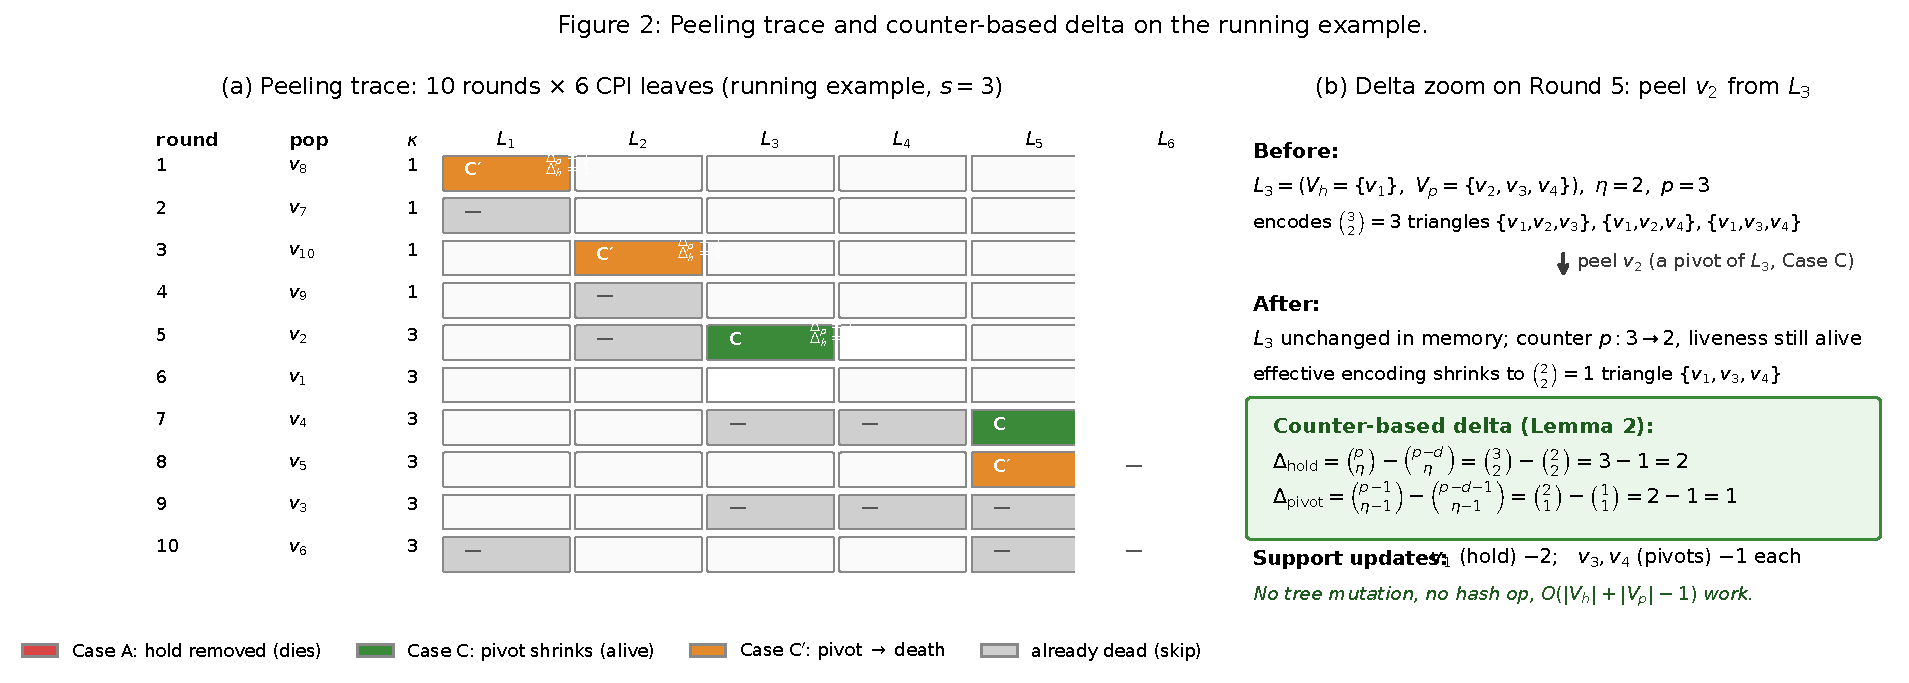
\includegraphics[width=\linewidth]{figures/fig2_peeling.pdf}
\caption{Event-driven peel on the running example.
%
Each row gives the popped vertex, its core value, and the path event under Theorem~\ref{thm:vertex-removal}.
%
The key distinction is that a hold peel kills a path, while a pivot peel only decreases \(p_{\mathcal{P}}\).
%
The \(\Delta_h\) and \(\Delta_p\) columns show the binomial losses from Lemma~\ref{lem:support-delta}.
%
The trace shows how mutable residual-index updates become path events and counter deltas.}
\Description{A peeling trace matrix for the running example, with color-coded path events and a zoomed binomial-delta calculation.}
\label{fig:peel}
\end{figure*}
